%%%%%%%%%%%%%%%%%%%%%%%%%%%%%%%%%%%%%%%%%%%%%%%%%%%%%%%%%%%%%%%%%%%%%%%%%%%%%%%
\section{DETAILED DESIGN AND REALIZATION}\label{sec:detailed_design}
%%%%%%%%%%%%%%%%%%%%%%%%%%%%%%%%%%%%%%%%%%%%%%%%%%%%%%%%%%%%%%%%%%%%%%%%%%%%%%%

AtlantikSolar (Fig. \ref{fig:AtlantikSolarCollage}) is a solar-powered Low-Altitude Long-Endurance(LALE) UAV designed and built at ETH Zurich for perpetual flight at $\varphi=45\degree N$ geographical latitude from April 21\textsuperscript{st} to August 21\textsuperscript{st}. Although its design is mostly dictated by the requirement for low level-flight power consumption, it provides means to mount an advanced optical and infrared sensor pod developed at ETH Zurich for use in autonomous search and rescue or industrial inspection missions. The airplane airframe characteristics are summarized in table \ref{tab:DetailedDesignParameters}. An overview over the airplane system topology is given in Fig. \ref{fig:AtlantikSolar_SystemOverview}.

\begin{figure}[h]
    \centering
    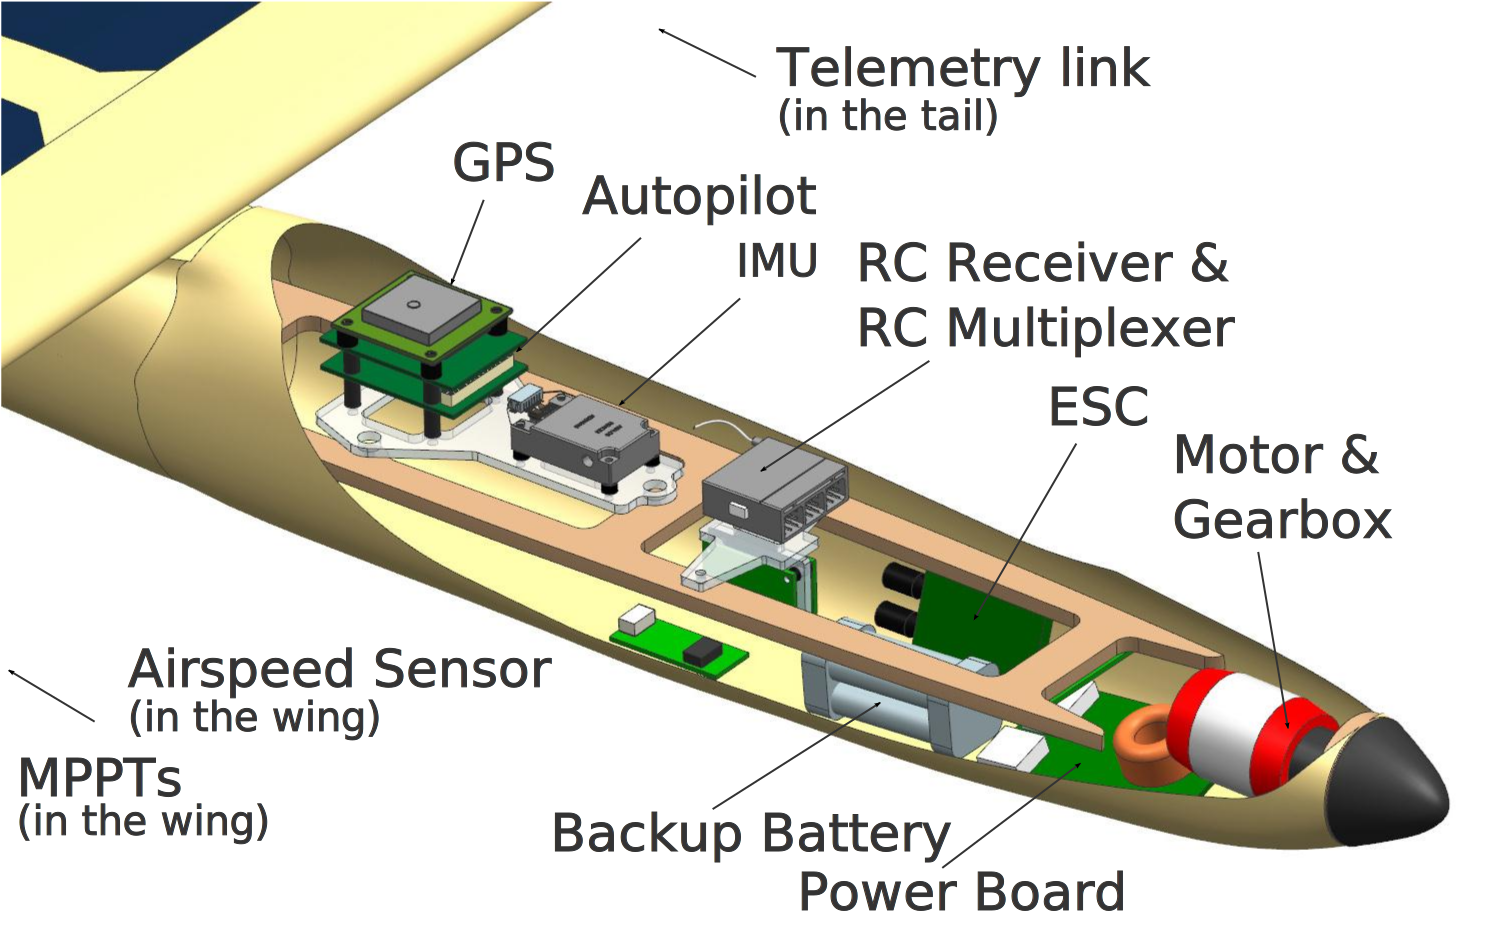
\includegraphics[width=\linewidth]{images/10_CAD_AtlantikSolarAvionicsCombined/10_CAD_AtlantikSolarAvionicsCombined}
    \caption{Left: Wing structure with integrated batteries and solar cells. Right: Main avionics layout inside the airplane.}
    \label{fig:CAD_AtlantikSolarStructureAndAvionics}
\end{figure}
%\begin{figure}[tb]
%    \centering
%    \includegraphics[width=\linewidth]{images/6_CAD_AtlantikSolarFull}
%    \caption{The AtlantikSolar UAV features a conventional T-tail configuration with 1 motor, two ailerons, an all-moving elevator and a rudder for actuation.}
%    \label{fig:CAD_AtlantikSolarFull}
%\end{figure}

\begin{table}
\caption{AtlantikSolar design characteristics}
\label{tab:DetailedDesignParameters}
\begin{center}
\begin{tabular}{l l}
Wing span & 5.65$\unit{m}$\\
\hline Wing chord& 0.305$\unit{m}$\\
\hline Length& 2.03\unit{m}\\
\hline Height&0.45\unit{m}\\
\hline Mass& 7.36$\unit{kg}$\\
\hline Battery mass& 3.52$\unit{kg}$\\
\hline Wing loading&4.28$\unitfrac{kg}{m^2}$\\
\hline Stall speed& 8.1$\unitfrac{m}{s}$\\
\end{tabular}
\end{center}
\end{table}

%%%%%%%%%%%%%%%%%%%%%%%%%%%%%%%%%%%%%%%%%%%%%%%%%%%%%%%%%%%%%%%%%%%%%%%%%%%%%%%
\subsection{UAV Platform Design}
%%%%%%%%%%%%%%%%%%%%%%%%%%%%%%%%%%%%%%%%%%%%%%%%%%%%%%%%%%%%%%%%%%%%%%%%%%%%%%%

%%%%%%%%%%%%%%%%%%%%%%%%%%%%%%%%%%%%%%%
\subsubsection{Airframe}\label{secsec:Airframe and hardware}
%%%%%%%%%%%%%%%%%%%%%%%%%%%%%%%%%%%%%%%
The wing and stabilizers of AtlantikSolar are built in a traditional rib-spar construction method (Fig. \ref{fig:CAD_AtlantikSolarStructureAndAvionics}). The wing's main element is an inner cylindrical carbon-fibre spar to resist torsional wing loads. Four carbon-fibre belts of trapezoidal and laterally-varying cross-section are attached to the spar to optimally resist bending loads and to provide maximum wing stiffness to avoid bending of the solar cells. The main wing can be disassembled into three wing pieces of $b<2m$ each.

%%%%%%%%%%%%%%%%%%%%%%%%%%%%%%%%%%%%%%%
\subsubsection{Energy Generation and Storage}
%%%%%%%%%%%%%%%%%%%%%%%%%%%%%%%%%%%%%%%
The cylindrical wing spars are fitted with 72 cylindrical high energy-density Lithium-Ion batteries (Panasonic NCR18650b, 243Wh/kg) to optimally distribute the mass in a \textit{span loader} concept. The cells are connected in a 6S (22.2V) configuration and provide $E_{bat,max}=850Wh$ at $m_{bat}=3.5kg$. The solar modules feature a total of 88 SunPower C60 cells with $\eta_{sm}=0.20$, an areal density of $k_{sm}=590g/m^2$ and a maximum power output of 275W at $\varphi=45\degree$ on June 21\textsuperscript{st}. Modules featuring SunPower E60 cells with $\eta_{sm}=0.23$ are currently being integrated\cite{Sunier_EPFLSolarModules}. The solar modules are seamlessly embedded in the upper wing surface to avoid premature flow separation.

\begin{figure}[tb]
    \centering
     \includegraphics[width=\linewidth]{images/8_AtlantikSolar_Avionics}
    \caption{AtlantikSolar system overview. For clarity, voltage lines from the autopilot to connected devices (5.0V and 3.3V) are omitted.}
    \label{fig:AtlantikSolar_SystemOverview}
\end{figure}

%%%%%%%%%%%%%%%%%%%%%%%%%%%%%%%%%%%%%%%
\subsubsection{Actuation}
%%%%%%%%%%%%%%%%%%%%%%%%%%%%%%%%%%%%%%%
The propulsion system features a foldable custom built carbon-fibre propeller with diameter $D=66cm$ and pitch $H=60cm$. It is driven by a 5:1 reduction-ratio planetary gearbox, a RS-E Strecker 260.20 brushless DC motor with $k_V=450RPM/V$ and a Kontronik Koby 55 LV motor controller at up to $P_{prop,max}=450W$ electrical input power. The actuation system consists of four Volz DA-15N servos that drive the two ailerons, the all-moving elevator and the rudder. To guarantee reliable multi-day flight, the Volz actuators were successfully operated in a servo test-bed for 30 days under flight-equivalent loads \cite{DellaCa_BT}.
%mention wind tunnel, lab motor test stand tests? Only if space left...

%%%%%%%%%%%%%%%%%%%%%%%%%%%%%%%%%%%%%%%
\subsubsection{Avionics} \label{secsec:Avionics}
%%%%%%%%%%%%%%%%%%%%%%%%%%%%%%%%%%%%%%%
The avionics installation (Figs. \ref{fig:AtlantikSolar_SystemOverview} and \ref{fig:CAD_AtlantikSolarStructureAndAvionics}) is centered around a Pixhawk PX4 Autopilot - an open source and open hardware project initiated at ETH Zurich - with a Cortex M4F microprocessor running at 168Mhz and featuring 192kB RAM. For attitude estimation (Sec. \ref{secsec:StateEstimation}), an ADIS 16448 10-axis Inertial Measurement Unit (IMU), a u-Blox LEA-6H GPS receiver, and a Sensirion SDP600 differential pressure sensor are used. The SDP600 airspeed sensor exhibits less than 5\% error at airspeeds of 8m/s, which is essential to closely track the minimum power $P_{out}$ airspeed. Both a 433Mhz medium-range telemetry link and a long-range IRIDIUM-based satellite backup link are integrated. The airplane implements a fully manual RC-command fall-back mode in case of a severe autopilot failure. Night operations are possible due to four on-board high-power indicator LEDs.

%%%%%%%%%%%%%%%%%%%%%%%%%%%%%%%%%%%%%%%
\subsubsection{Payload}
%%%%%%%%%%%%%%%%%%%%%%%%%%%%%%%%%%%%%%%
% [THOMAS]
The capabilities of AtlantikSolar are augmented by a sensor and processing unit which may be mounted beneath the wing. It incorporates a \emph{visual-inertial sensor system} \cite{nikolic2014synchronized} and a small form factor computer based on an Intel Atom processor. The former consists of an ARM-FPGA system, an ADIS 16448 IMU as well as two cameras - a FLIR Tau 2 for long-wavelength infrared (LWIR) and an Aptina MT9V034 for visible light imaging - and allows accurate real-time SLAM\cite{Leutenegger_PhD}. The latter is intended for high-level path planning and equipped with WiFi-communication to transmit a video feed to the ground.

%\begin{figure}[!htb]
%  \begin{center}
%  \def\svgwidth{\columnwidth}
%  \includesvg{pod}
%  \end{center}
%  \caption[Modular sensing and processing unit.]{Sensing and processing unit for integration below the wing.}
%  \label{f:03_sensor_pod}
%\end{figure}
\begin{figure}[tb]
    \centering
     \includegraphics[width=\linewidth]{images/pod}
    \caption[Modular sensing and processing unit.]{Sensing and processing unit for integration below the wing.}
    \label{f:03_sensor_pod}
\end{figure}

%%%%%%%%%%%%%%%%%%%%%%%%%%%%%%%%%%%%%%%%%%%%%%%%%%%%%%%%%%%%%%%%%%%%%%%%%%%%%%%
\subsection{State Estimation and Control Design}
%%%%%%%%%%%%%%%%%%%%%%%%%%%%%%%%%%%%%%%%%%%%%%%%%%%%%%%%%%%%%%%%%%%%%%%%%%%%%%%

%%%%%%%%%%%%%%%%%%%%%%%%%%%%%%%%%%%%%%%
\subsubsection{State Estimation} \label{secsec:StateEstimation}
%%%%%%%%%%%%%%%%%%%%%%%%%%%%%%%%%%%%%%%

The on-board state estimator is based on an extended Kalman filter (EKF) design that fuses data from the 10-axis IMU, GPS and airspeed sensor as described in Sec. \ref{secsec:Avionics}. It is implemented and optimized in order to grant full functionality on the microcontroller-based autopilot and offers a robust estimation solution that can cope with prolonged GPS outage scenarios by compensating through airspeed measurements. Successive estimations of the position, velocity, orientation (attitude and heading), QFF, gyroscopes biases, accelerometers biases and the wind vector are rendered, with sideslip angle and angle of attack (AoA) being subsequently derived from these estimates. A detailed description and verification of the state estimator functionality can be found in \cite{Leutenegger_MSC2014}.
  
%\begin{figure}[tb]
%    \centering
%    \includegraphics[width=\linewidth]{images/10_real_time_state_estimator_position}
%    \caption{Overhead trajectories plot of the on-board position state estimation (green) and the GPS  (black).}
%    \label{fig:real_time_state_estimator_positionl}
%\end{figure}


%%%%%%%%%%%%%%%%%%%%%%%%%%%%%%%%%%%%%%%
\subsubsection{System Identification} \label{sec:SystemID}
%%%%%%%%%%%%%%%%%%%%%%%%%%%%%%%%%%%%%%%
%[DR. ALEXIS] 
 %	This subsection overviews the system identification methods employed for AtlantikSolar

Towards aiding the control synthesis procedure, a simplified linear state--space representation of the UAV dynamics was also derived based on recorded flight data and frequency--domain system identification methods. For non--aggressive maneuvering and around level flight, linear models may capture the vehicle response for small perturbations around a given equilibrium. Decoupling the longitudinal and lateral axis the dynamics of a UAV may take the following form~\cite{dorobantu2011frequency,OMLAS_MED_2014}: 

\small
\begin{eqnarray}\label{LON_DYN}
 \mathbf{M}_{lon}\dot{\mathbf{x}}_{lon} &=& \mathbf{A}^\prime_{lon}\mathbf{x}_{lon}+\mathbf{B}^\prime_{lon}u_{elev} \\ \nonumber
 \mathbf{x}_{lon} &=& \left[ u~w~q~\theta \right]^T
\end{eqnarray}
\normalsize
where $u,w,q,\theta$ correspond to the body $x$--axis, $z$--axis velocities, the pitch rate and the pitch angle respectively, $u_{elev}$ corresponds to the elevator deflection and

\scriptsize
\begin{eqnarray}
\mathbf{M}_{lon} &=& \begin{bmatrix}
m & 0 & 0 & 0\\ 
0 & m & 0 & 0\\ 
0 & 0 & I_y & 0\\ 
0 & 0 & 0 & 1
\end{bmatrix},\\ \nonumber
\mathbf{A}^\prime_{lon} &=& \begin{bmatrix}
X_u & X_w & X_q-mW_e & -mg\cos\theta_e\\ 
Z_u & Z_w & Z_q+mU_e & -mg\sin\theta_e\\ 
M_u & M_w & M_q & 0 \\ 
0 & 0 & 1 & 0
\end{bmatrix}~
\mathbf{B}^\prime_{lon} = \begin{bmatrix}
X_{u_{elev}}\\ 
Z_{u_{elev}}\\ 
M_{u_{elev}}\\ 
0
\end{bmatrix}
\end{eqnarray}
\normalsize
where $m$ is the mass, $I_y$ the inertia around the body $y$--axis, $W_e,\theta_e$ are the trimming points of vertical velocity and pitch angle, and the elements of $\mathbf{M}_{lon},\mathbf{A}^\prime_{lon}$ and $\mathbf{B}^\prime_{lon}$ form the stability and control derivatives of the UAV longitudinal dynamics. 

Similarly, for the lateral dynamics the model takes the following form:


\small
\begin{eqnarray}\label{LAT_DYN}
 \mathbf{M}_{lat}\dot{\mathbf{x}}_{lat} &=& \mathbf{A}^\prime_{lat}\mathbf{x}_{lat}+\mathbf{B}^\prime_{lat}u_{elev} \\ \nonumber
 \mathbf{x}_{lat} &=& \left[v~p~r~\phi \right]^T
\end{eqnarray}
\normalsize
where $v,p,r,\phi$ correspond to the body $y$--axis velocity, the roll and yaw rates and roll angle respectively, $u_{ail}$ is the aileron deflection, $u_{rud}$ is the rudder deflection and

\scriptsize
\begin{eqnarray}
\mathbf{M}_{lat} &=& \begin{bmatrix}
m & 0 & 0 & 0\\ 
0 & I_x & -I_{xz} & 0\\ 
0 & -I_{xz} & I_z & 0\\ 
0 & 0 & 0 & 1
\end{bmatrix},\\ \nonumber 
\mathbf{A}^\prime_{lat} &=& \begin{bmatrix}
Y_v & Y_p + mW_e & Y_r-mU_e & mg\cos\theta_e\\ 
L_v & L_p & L_r & 0\\ 
N_v & N_p & N_r & 0 \\ 
0 & 1 & \tan\theta_e & 0
\end{bmatrix},~ \mathbf{B}^\prime_{lat} = \begin{bmatrix}
Y_{u_{ail}} & Y_{u_{rud}}\\ 
L_{u_{ail}} & L_{u_{rud}}\\ 
N_{u_{ail}} & N_{u_{rud}}\\ 
0 & 0
\end{bmatrix}
\end{eqnarray}
\normalsize
where $I_x$ the inertia around the body $x$--axis, $I_{xz}$ the cross--inertia term of the body $x,z$--axes and the elements of $\mathbf{M}_{lat},\mathbf{A}^\prime_{lat}$ and $\mathbf{B}^\prime_{lat}$ form the stability and control derivatives of the UAV lateral dynamics. 
 
 %%%%%%%%%%%%%%%%%%%%%%%%%%%%%%%%%%%%%%%
 \subsubsection{Control} \label{sec:Control}
 %%%%%%%%%%%%%%%%%%%%%%%%%%%%%%%%%%%%%%%
 %[PHILIPP writes this, DR. ALEXIS checks this]

 %	This subsection provides some info on the controllers that run on AtlantikSolar

\begin{figure}[tb]
    \centering
     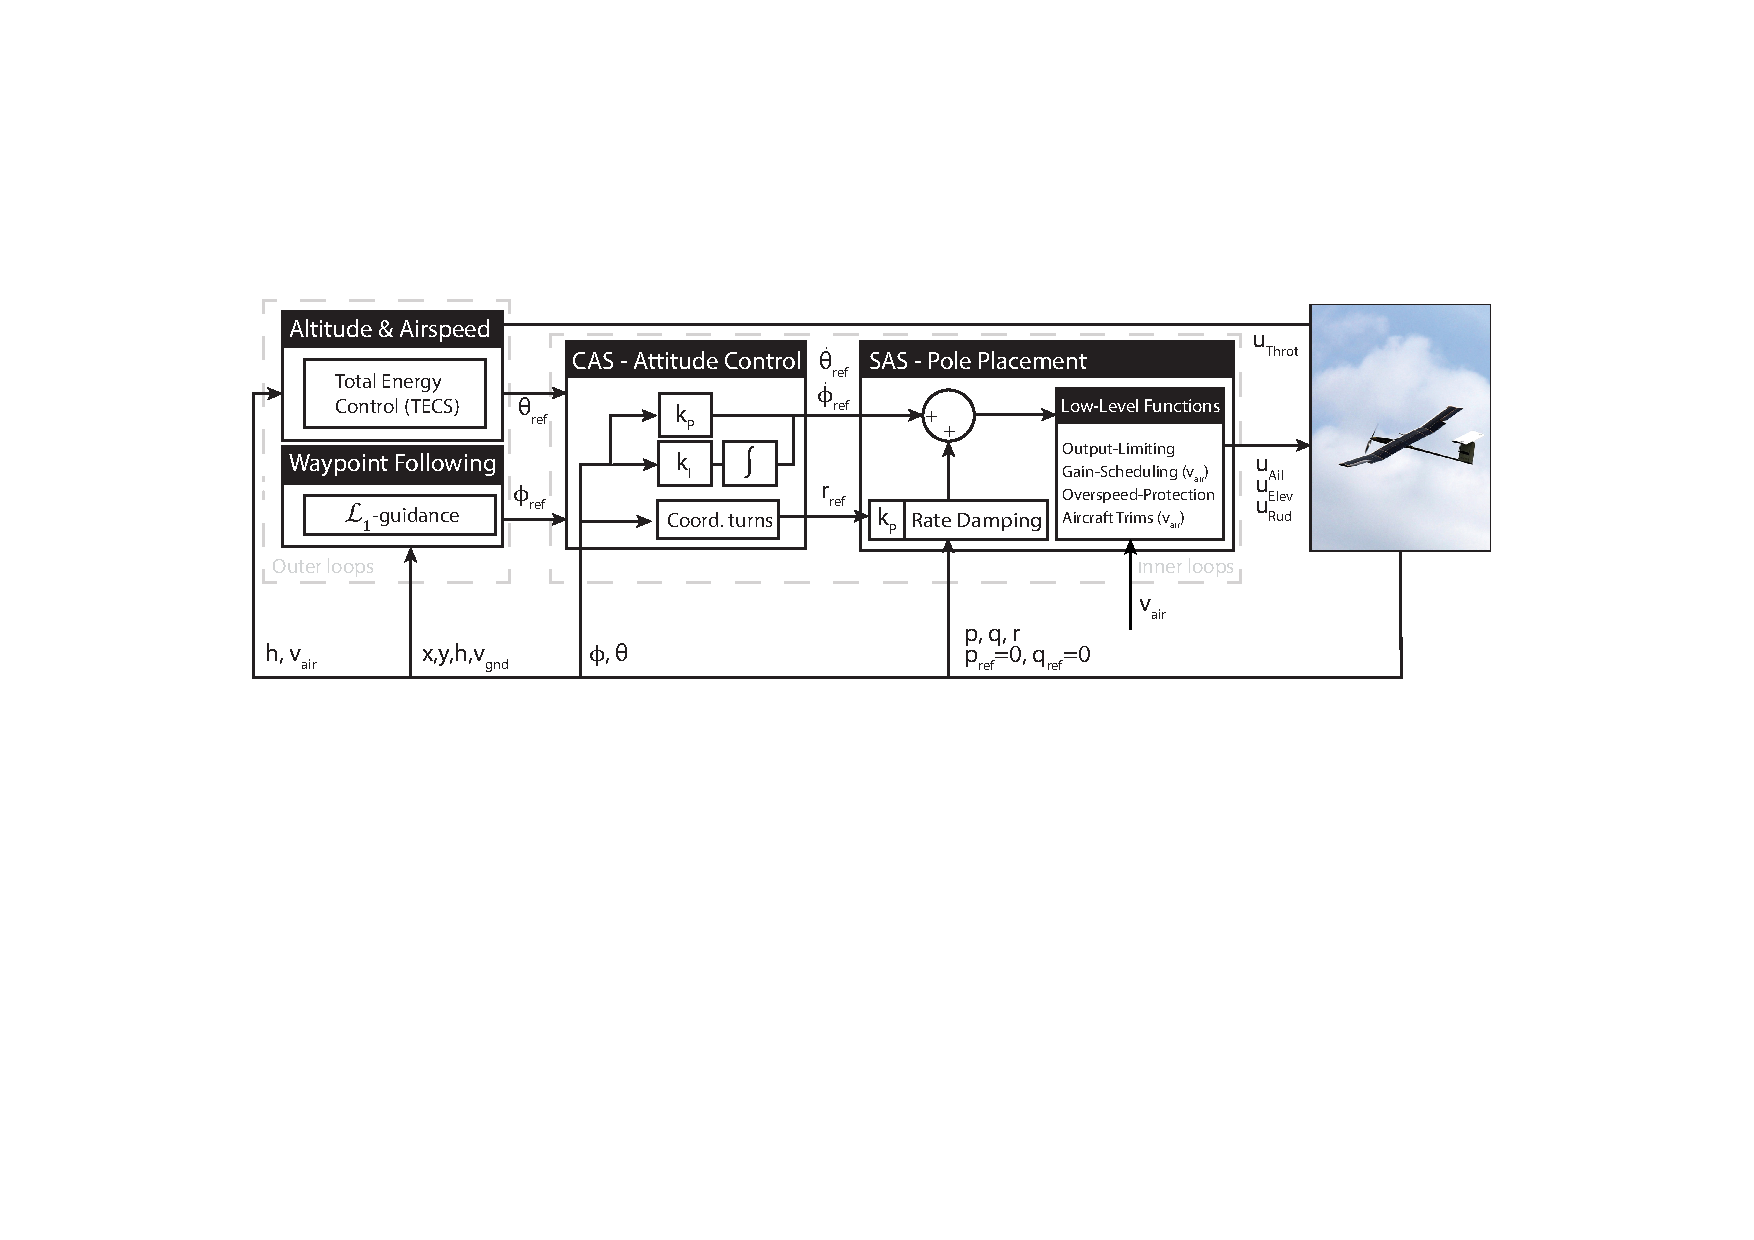
\includegraphics[width=\linewidth]{images/11_ControlScheme/ControlScheme.pdf}
    \caption{Control Scheme implemented for AtlantikSolar.}
    \label{fig:ControlScheme}
\end{figure}

AtlantikSolar features autonomous navigation and loitering through user--defined waypoints. The complete control structure (Fig.~\ref{fig:ControlScheme}) is offline-tuned based on the identified system model (Sec.~\ref{sec:SystemID}), functionality-tested in an X--Plane 10 Hardware--In--the--Loop (HIL) simulation and finally refined in extensive flight tests. For inner--loop control, our baseline--solution corresponds to a set of cascaded saturated PID controllers: The Stability Augmentation System (SAS) applies rate--damping to shape the airplane's frequency response, while the Control Augmentation System (CAS) applies proportional--integral feedback to achieve roll ($\phi$) and pitch ($\theta$) reference tracking. As a cascaded approach, proper tuning requires iteration of the gains to achieve maximum performance and robustness against model uncertainties and external disturbances. Flight tests showed that due to AtlantikSolar's high wingspan and thus high x- and z-axis inertia $I_x$ and $I_z$, coordinated turn control is essential to damp adverse yaw and to achieve the no--sidelslip yaw rate $r=\frac{g\cdot \sin(\phi)}{v_{air}}$. To avoid overload of the highly optimized structure, output limiters and an over--speed protection are applied. Furthermore, the control actions are in a final stage adapted with respect to the dynamic pressure $q=\frac{1}{2}\rho v^{2}_{air}$ which accounts for the change of the effective moments created by the control surfaces. 

Once the inner--loops are well--tuned, waypoint guidance is enabled. AtlantikSolar employs a $\mathcal{L}_1$--nonlinear guidance law which generates the lateral acceleration reference $a_{s_{ref}}$ of the UAV based on a look--ahead distance ${L}_1$ and the current velocity $V_T$ and heading error $\eta$ as noted below:

\small
\begin{eqnarray}
 a_{s_{ref}} &=& 2\frac{V_T^2}{L_1}\sin \eta
\end{eqnarray}
\normalsize
which is then kinematically translated to roll references while consistent dynamic behaviour is achieved via adaptation of the look--ahead distance as in~\cite{L1stabAnalysis}. This guidance law is integrated into our control structure as described in~\cite{OMLAS_MED_14} and combined with an extended version of the Pixhawk open--source Total Enery Control System (TECS)~\cite{PixhawkWebsite} which provides altitude control: First, a slew rate constraint on the reference altitude $h_{ref}$ has been integrated to reach smoother altitude control at pre-definable climb and sink rates, which is especially important for low propulsion-power to weight-ratio UAVs such as AtlantikSolar. Second, we have implemented \textit{thermal compliance}: In an updraft, the standard TECS implementation will decrease $\theta_{ref}$ to decrease the altitude if $h>h_{ref}$. To allow gaining potential energy from a thermal, we perform gain-scheduling on TECS configuration parameters such that $\theta_{ref}$ is used only for airspeed control and $u_{Throt}$ only for altitude control. When at $h>h_{ref}$, the plane will thus keep $\theta_{ref}=\theta_{ref}(t)$  such that $v(t)=v_{ref}(t)$ and will gradually disable the motor, potentially gaining altitude for strong thermals. Furthermore, altitude limits have been implemented, i.e. full throttle is forced for $h<h_{min}$, at $h>h_{max}$ we gradually allow a pitch-down and thus altitude decrease again, and at $h>h_{max}+50m$ the controller automatically engages the spoilers for maximum descend rate. The inner PID-based pitch- and roll control loops are executed at a sampling period of $T_{SAS,CAS}=0.01s$, while the high-level $\mathcal{L}_1$\&TECS controllers run with $T_{\mathcal{L}_1,TECS}=0.05s$. Given these settings, the full controller requires less than 4\% CPU load, 5KB of RAM and 47KB Flash memory and is thus computationally lightweight when compared to other Pixhawk applications (see~\cite{OMLAS_MED_14}) such as the state estimation. The whole control application is designed to be modular, and more sophisticated approaches like model-predictive control~\cite{OMLAS_MED_14} and robust $H_\infty$--based controllers~\cite{Mosimann_FT} for inner loop control have been implemented and flown on test planes in addition to our cascaded PID baseline-solution. 
